\documentclass[11pt]{article}  
\usepackage[margin=1in]{geometry}
\parindent=0in
\parskip=8pt
\usepackage{fancyhdr,amssymb,amsmath, graphicx, listings,float,subfig,enumerate,epstopdf,color,multirow,setspace,bm,textcomp}
\usepackage[usenames,dvipsnames]{xcolor}
\usepackage{hyperref}
\usepackage{graphicx}
\graphicspath{{./Images}}

\pagestyle{fancy}


\begin{document} 

\lhead{Assignment \#  6}
\chead{Robert Denim Horton}
\rhead{\today}

\begin{center}\begin{Large}
CS 4740 Networks, Crowds, and Markets 

Homework \# 6

Student: (Robert Denim Horton)
\end{Large}
\end{center}

\section*{Answers to homework problems:}

% Question 1
\begin{enumerate}
	\item Say whether the following claim is true or false, and provide a brief (1-3 sentence) explanation for your answer. \\
	\begin{quote}
		 Claim: If player A in a two-person game has a dominant strategy $s_A$, then there is a pure strategy Nash equilibrium in which player A plays $s_A$ and player B plays a best response to $s_A$. 
	\end{quote}
\end{enumerate}
% Question 1 Answers
\textcolor{gray}{
Answers:
\begin{enumerate}
	\item Well, it is known that since player A has a dominant strategy the player A's strategy will always have a higher value than player B regardless of what ever decision player B makes.  We also know that there to be Nash equilibrium then there exists a best outcome that either player can experience dependent of what ever decision the other player, B,  makes. However,  player A has a dominant strategy and means that both players are not guaranteed to make decision resulting in Nash equilibrium.   
\end{enumerate}
}

% Question 3
\begin{enumerate}
	\setcounter{enumi}{2}
	\item Find all pure strategy Nash equilibria in the game below. In the payoff matrix below the rows correspond to player A’s strategies and the columns correspond to player B’s strategies. The first entry in each box is player A’s payoff and the second entry is player B’s payoff.
	\begin{center}
		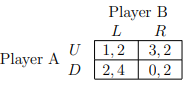
\includegraphics[scale=1.0]{Figure1.1}
	\end{center}
\end{enumerate}
% Question 3 Answers
\textcolor{gray}{
Answers:
\begin{enumerate}
	\setcounter{enumi}{2}
	\item Fomaily defing Nash equilibirum, the book says, ". . . suppose that Player 1 chooses a strategy S and Player 2 chooses a strategy T.  We say that this pair of strategies, (S, T), is a Nash equilibrium if S is a best response to T, and T is a best response to S.  
	\item  Below is a table made to show best results for row and coumn choices from the playoff matrix.\\
	\begin{center}
		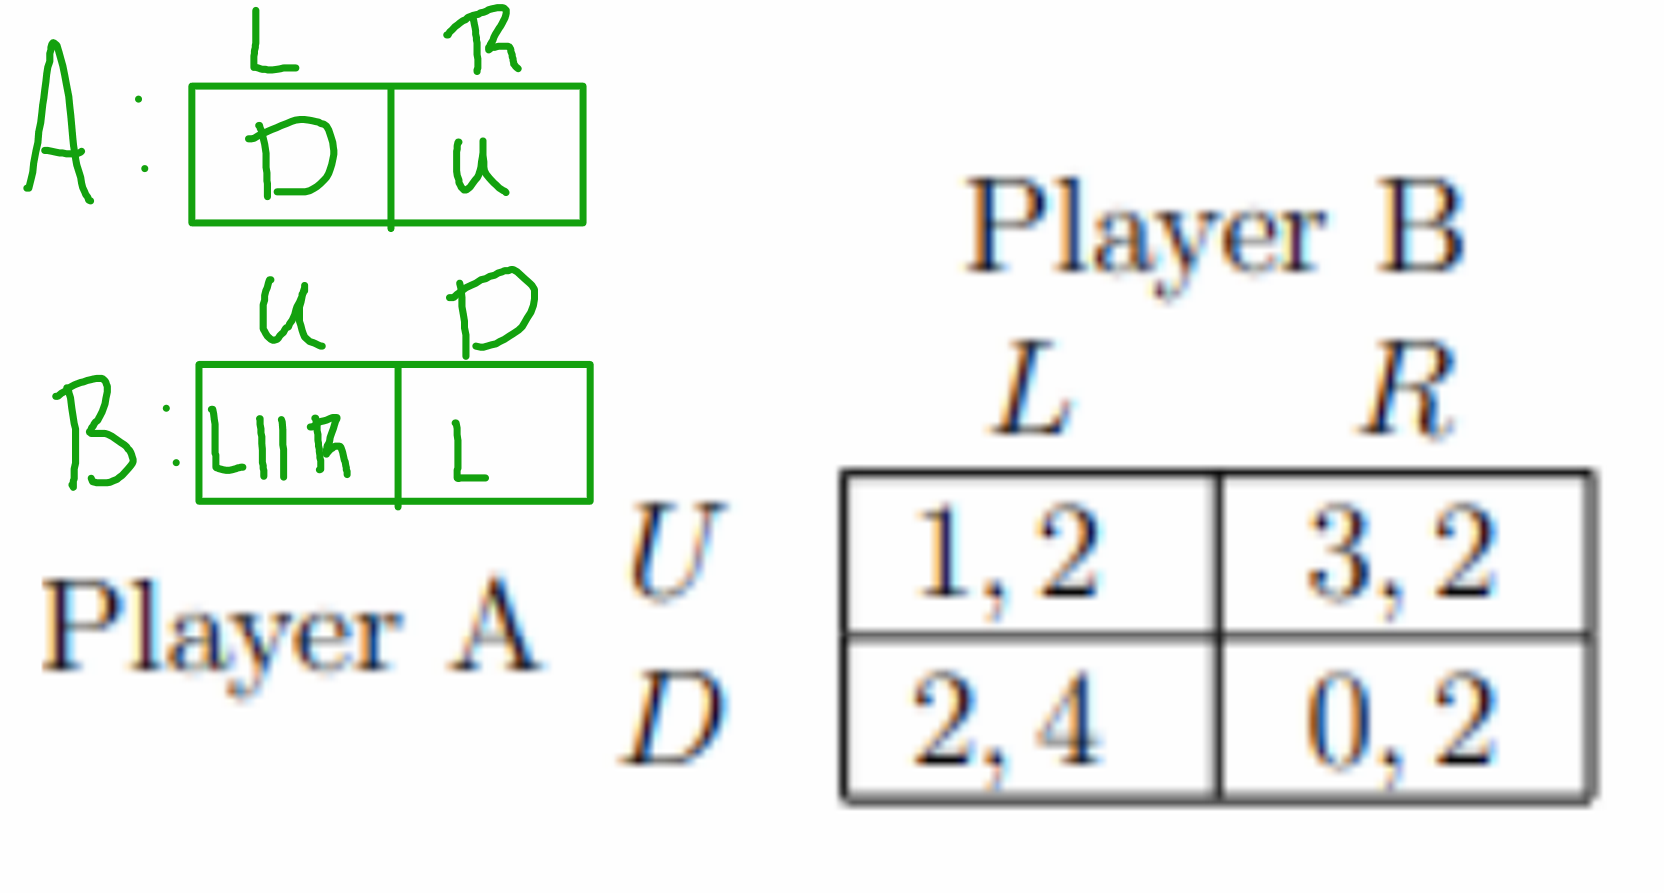
\includegraphics[scale=0.3]{Figure1.4}\\
	\end{center}
To begin finding all the Nash equilibria we will simply evaluate the best strategy for each player depending on which action the other player performs.\\\\
	So first evaluating player A's best strategy we know that if player B chooses column L then player A must choose row D because 2 is better than 1. If player B chooses coloumn R then player A's best choice would be row U since 3 is greater then 0.\\\\
 	Now evaluating Player B's best stratey, we know that if player A chooses Row D then player B's best choice is to pick coumn L because 4 is better than 2.  When Player A chooses column U, then player B can chooses either choice and get the same reward of 2.\\\\
So, we can classify the best possible out comes for both players as;\\
\begin{itemize}
	\item Player A chooses U and player B chosses R\\
	\item Player A chooses D and player B chosses L\\
\end{itemize}
These pairs of combined choices, $(U, \ R)$ and $(D, \ L)$ can be considered as Nash equilibirum since either one of them would be a best response to what ever choice the other player might make.
\end{enumerate}
}

% Question 4
\begin{enumerate}
	\setcounter{enumi}{3}
	\item  Consider the two-player game with players, strategies and payoffs described in the following game matrix.
	\begin{center}
		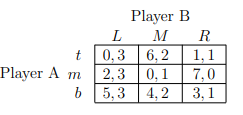
\includegraphics[scale=1.0]{Figure1.2}
	\end{center}
	\begin{enumerate}[(a)]
		% Question 4: Part 1
		\item Does either player have a dominant strategy? Explain briefly (1-3 sentences).
		% Question 4: Part 2
		\item Find all pure strategy Nash equilibria for this game.
	\end{enumerate}
\end{enumerate}
% Question 4 Answers
\textcolor{gray}{
Answers:
\begin{enumerate}
	\setcounter{enumi}{3}
	\item  Below is a table made to show best results for row and coumn choices from the playoff matrix.
	\begin{center}
		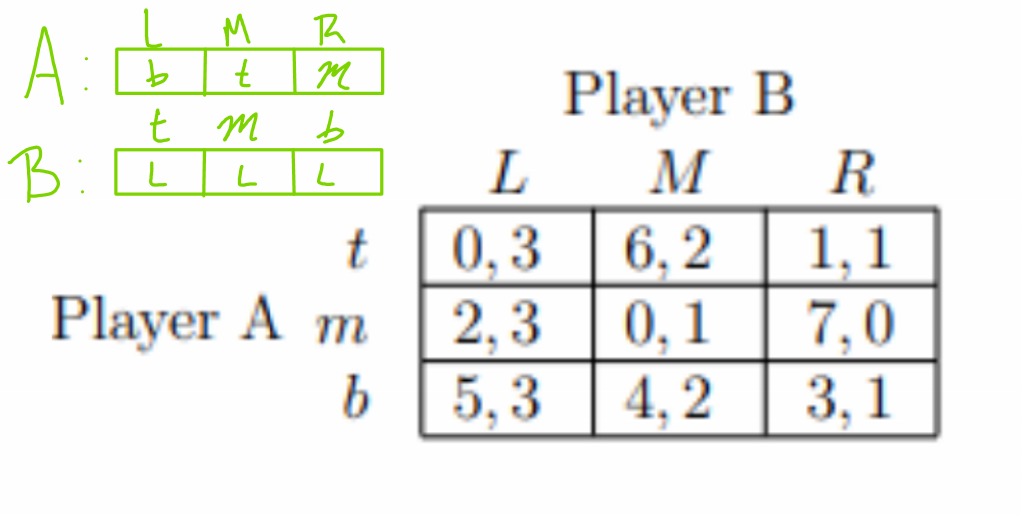
\includegraphics[scale=0.65]{Figure1.5}
	\end{center}
	\begin{enumerate}[(a)]
		% Question 4: Part 1
		\item Considering each players best strategy we can evaluate each scenario of choices made by both players.\\\\
		When considering players A's best strategy we look at the all the moves player B can choose and then pick palyer A's best choice acordingly. If player B chooses $L$ then player A's best choice will be any of the choices $b$ becuase 5 is greater than 2 and 0. If player B chooses $M$ then player A's best choice will be $t$ since 6 is the greatest reward. If player B chooses $R$ then player A's best choice will be $m$ since 7 is greater than 3 and 1.\\\\
		When considering players B's best strategy we look at the all the moves player A can choose and pick palyer B's best choice acordingly.  If player A chooses $t$ then player B's best choice will be $L$ since 3 is greater than 2 or 1. If player A chooses $m$ then player B's best choice will once again be $L$ since 3 is greater then 1 and 0. If player A chooses $b$ then player B's best choice will be $L$ again because 3 is greater than 2 and 1.\\\\
As we can see reagardless of what action players A makes player B will always choose $L$.  From this we can say that player B has a dominant strategy, $L$.
		% Question 4: Part 2
		\item Continuing off the information that was gathered in part (a), we found that a Nash equilibrium , $(B, \ L)$, occours when player A chooses $b$ and player B chooses $L$ since both values return values from these choices sum to 8 being the highest total return amongst players.
	\end{enumerate}
\end{enumerate}
}

% Question 5
\begin{enumerate}
	\setcounter{enumi}{4}
	\item Consider the following two-player game in which each player has three strategies.\\
	\begin{center}
		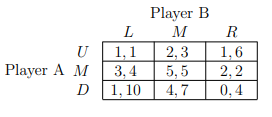
\includegraphics[scale=1.0]{Figure1.3}\\
	\end{center}
	Find all the (pure strategy) Nash equilibria for this game.\\
\end{enumerate}
% Question 5 Answers
\textcolor{gray}{
Answers:
\begin{enumerate}
	\setcounter{enumi}{4}
	\item  Below is a table made to show best results for row and coumn choices from the playoff matrix.\\
	\begin{center}
		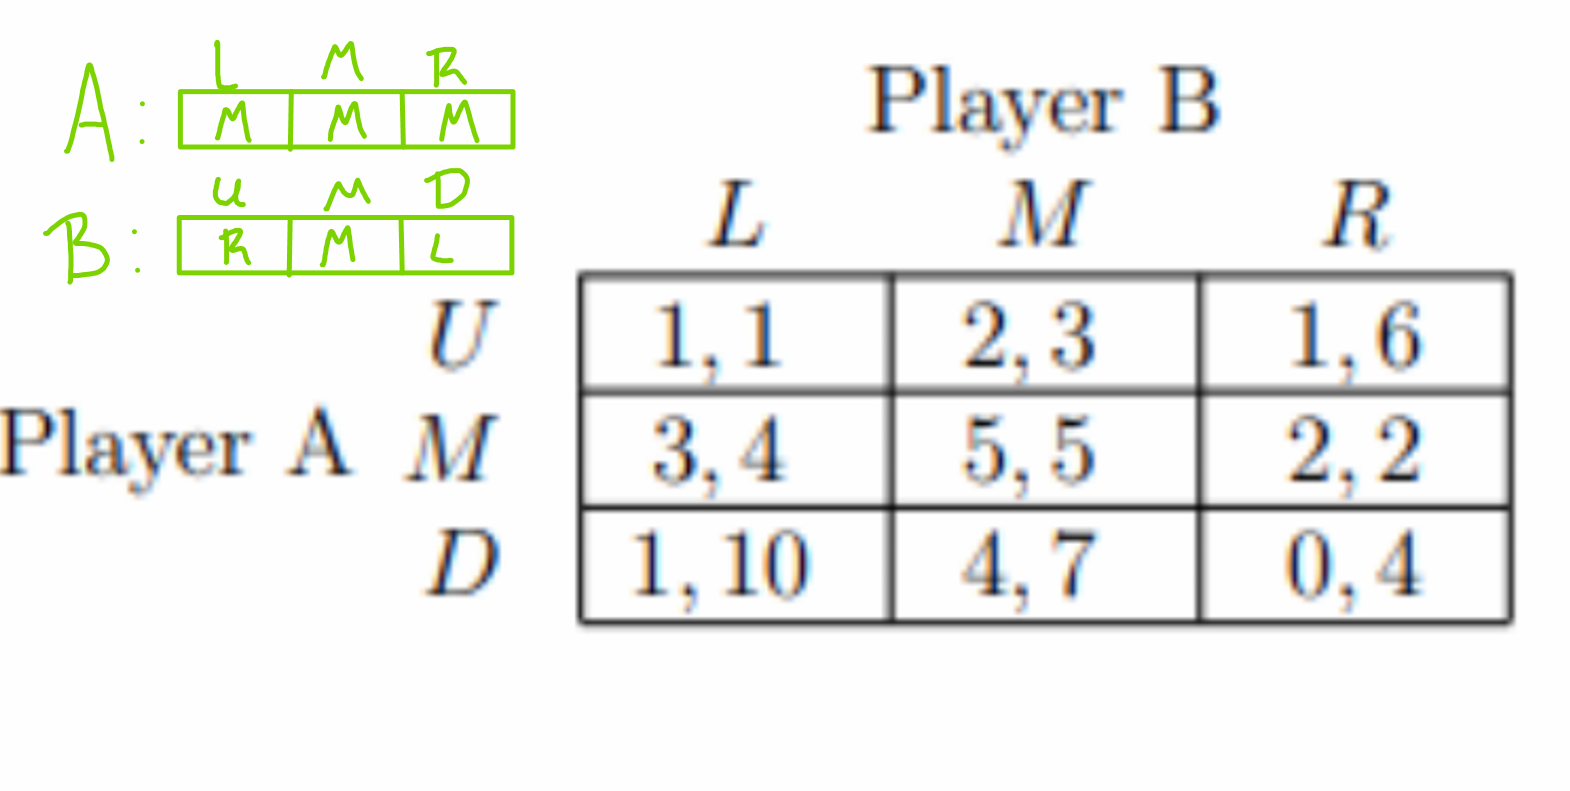
\includegraphics[scale=0.45]{Figure1.6}\\
	\end{center}
	For Player A's best strategy, if player B chooses $L$ then player A must choose $M$ since 3 is greater than 1. If player B chooses $M$ then palyer A must choose $M$ since 5 is greater than 4 and 2.   If player B chooses $R$ then palyer A must choose $M$ since 2 is greater than 0 and 1.\\\\
	For Player B's best strategy, if player A chooses $U$ then player B must choose $R$ since 6 is greater than 3 and 1. If player A chooses $M$ then palyer B must choose $M$ since 5 is greater than 4 and 2.   If player B chooses $R$ then palyer A must choose $L$ since 10 is greater than 4 and 1.\\\\  
Hence, we can see that move $M$ for both players result in a Nash equilibirum since this would be the best response to either one of the players moves. 
\end{enumerate}
}
\end{document}
